\chapter{Исследовательский раздел}
В данном разделе описана методика нагрузочного тестирования
реализованного многопоточного HTTP-сервера,
приведены результаты экспериментов
и сформулированы выводы о выборе оптимальной конфигурации.

\section{Условия проведения исследования}
Нагрузочное тестирование проводилось с помощью утилиты wrk,
которая генерирует HTTP-запросы в многопоточном режиме.

Тестирование проводилось на машине со следующими характеристиками:
\begin{itemize}
	\item операционная система Ubuntu 22.04.5 LTS;
	\item объем оперативной памяти - 56 ГБ;
	\item объем свободного пространства NVME2 накопителя Samsung 980 EVO —
500 ГБ [9];
	\item процессор Intel Core i9-11900KF @ 3.50 GHz
\end{itemize}

Параметры исследования:
\begin{itemize}
	\item количество потоков wrk: 8;
	\item длительность каждого прогона: 3 секунды;
	\item количество прогонов на каждую комбинацию параметров: 10;
	\item запрашиваемый ресурс: статическая HTML-страница;
	\item уровни одновременных подключений: 10\,000, 20\,000, 40\,000, 80\,000, 100\,000.
\end{itemize}



Тестировались шесть конфигураций сервера,
различающихся количеством потоков-слушателей ($L$)
и потоков-обработчиков ($W$):
$(L{=}2,\,W{=}2)$,
$(L{=}2,\,W{=}4)$,
$(L{=}2,\,W{=}8)$,
$(L{=}3,\,W{=}4)$,
$(L{=}3,\,W{=}8)$,
$(L{=}4,\,W{=}4)$.

Для каждой комбинации параметров вычислялись средние значения
трёх метрик: количество запросов в секунду (req/s),
средняя задержка ответа (мс) и скорость передачи данных (МБ/с).

\section{Результаты тестирования}
В таблице~\ref{tab:benchmark} приведены усреднённые результаты
нагрузочного тестирования по всем конфигурациям и уровням нагрузки.

\begin{table}[H]
\centering
\caption{Результаты нагрузочного тестирования (средние значения)}
\label{tab:benchmark}
\begin{tabular}{|c|c|c|c|c|c|}
\hline
$L$ & $W$ & Подключения & Запросов/с & Задержка, мс & Передача, МБ/с \\
\hline
2 & 2 & 10\,000 & 95\,247 & 99,15 & 868,9 \\
\hline
2 & 2 & 20\,000 & 48\,090 & 122,82 & 438,4 \\
\hline
2 & 2 & 40\,000 & 2\,569 & 30,80 & 23,5 \\
\hline
2 & 2 & 80\,000 & 927 & 31,10 & 8,5 \\
\hline
2 & 2 & 100\,000 & 709 & 30,80 & 6,5 \\
\hline
2 & 4 & 10\,000 & 150\,154 & 63,12 & 1\,369,1 \\
\hline
2 & 4 & 20\,000 & 65\,770 & 86,19 & 599,7 \\
\hline
2 & 4 & 40\,000 & 3\,450 & 24,49 & 31,5 \\
\hline
2 & 4 & 80\,000 & 1\,240 & 24,30 & 11,3 \\
\hline
2 & 4 & 100\,000 & 924 & 24,85 & 8,4 \\
\hline
2 & 8 & 10\,000 & 168\,414 & 56,79 & 1\,535,0 \\
\hline
2 & 8 & 20\,000 & 71\,480 & 68,83 & 651,8 \\
\hline
2 & 8 & 40\,000 & 3\,726 & 23,45 & 34,0 \\
\hline
2 & 8 & 80\,000 & 1\,314 & 23,80 & 12,0 \\
\hline
2 & 8 & 100\,000 & 1\,001 & 23,70 & 9,1 \\
\hline
3 & 4 & 20\,000 & 68\,303 & 75,80 & 622,8 \\
\hline
3 & 4 & 40\,000 & 3\,535 & 23,90 & 32,3 \\
\hline
3 & 4 & 80\,000 & 1\,185 & 25,25 & 10,8 \\
\hline
3 & 4 & 100\,000 & 922 & 23,90 & 8,4 \\
\hline
3 & 8 & 20\,000 & 68\,446 & 61,29 & 624,1 \\
\hline
3 & 8 & 40\,000 & 3\,604 & 23,85 & 32,9 \\
\hline
3 & 8 & 80\,000 & 1\,251 & 23,74 & 11,4 \\
\hline
3 & 8 & 100\,000 & 982 & 24,28 & 9,0 \\
\hline
4 & 4 & 10\,000 & 110\,845 & 103,18 & 1\,008,5 \\
\hline
4 & 4 & 20\,000 & 24\,028 & 212,69 & 219,1 \\
\hline
4 & 4 & 40\,000 & 2\,378 & 35,98 & 21,7 \\
\hline
4 & 4 & 80\,000 & 970 & 34,26 & 8,9 \\
\hline
\end{tabular}
\end{table}

\section{Исследование влияния количества потоков на пропускную способность}
На рисунке~\ref{fig:3d_rps} представлена зависимость количества
обработанных запросов в секунду от числа слушателей и обработчиков
для трёх уровней нагрузки.

\begin{figure}[H]
	\center{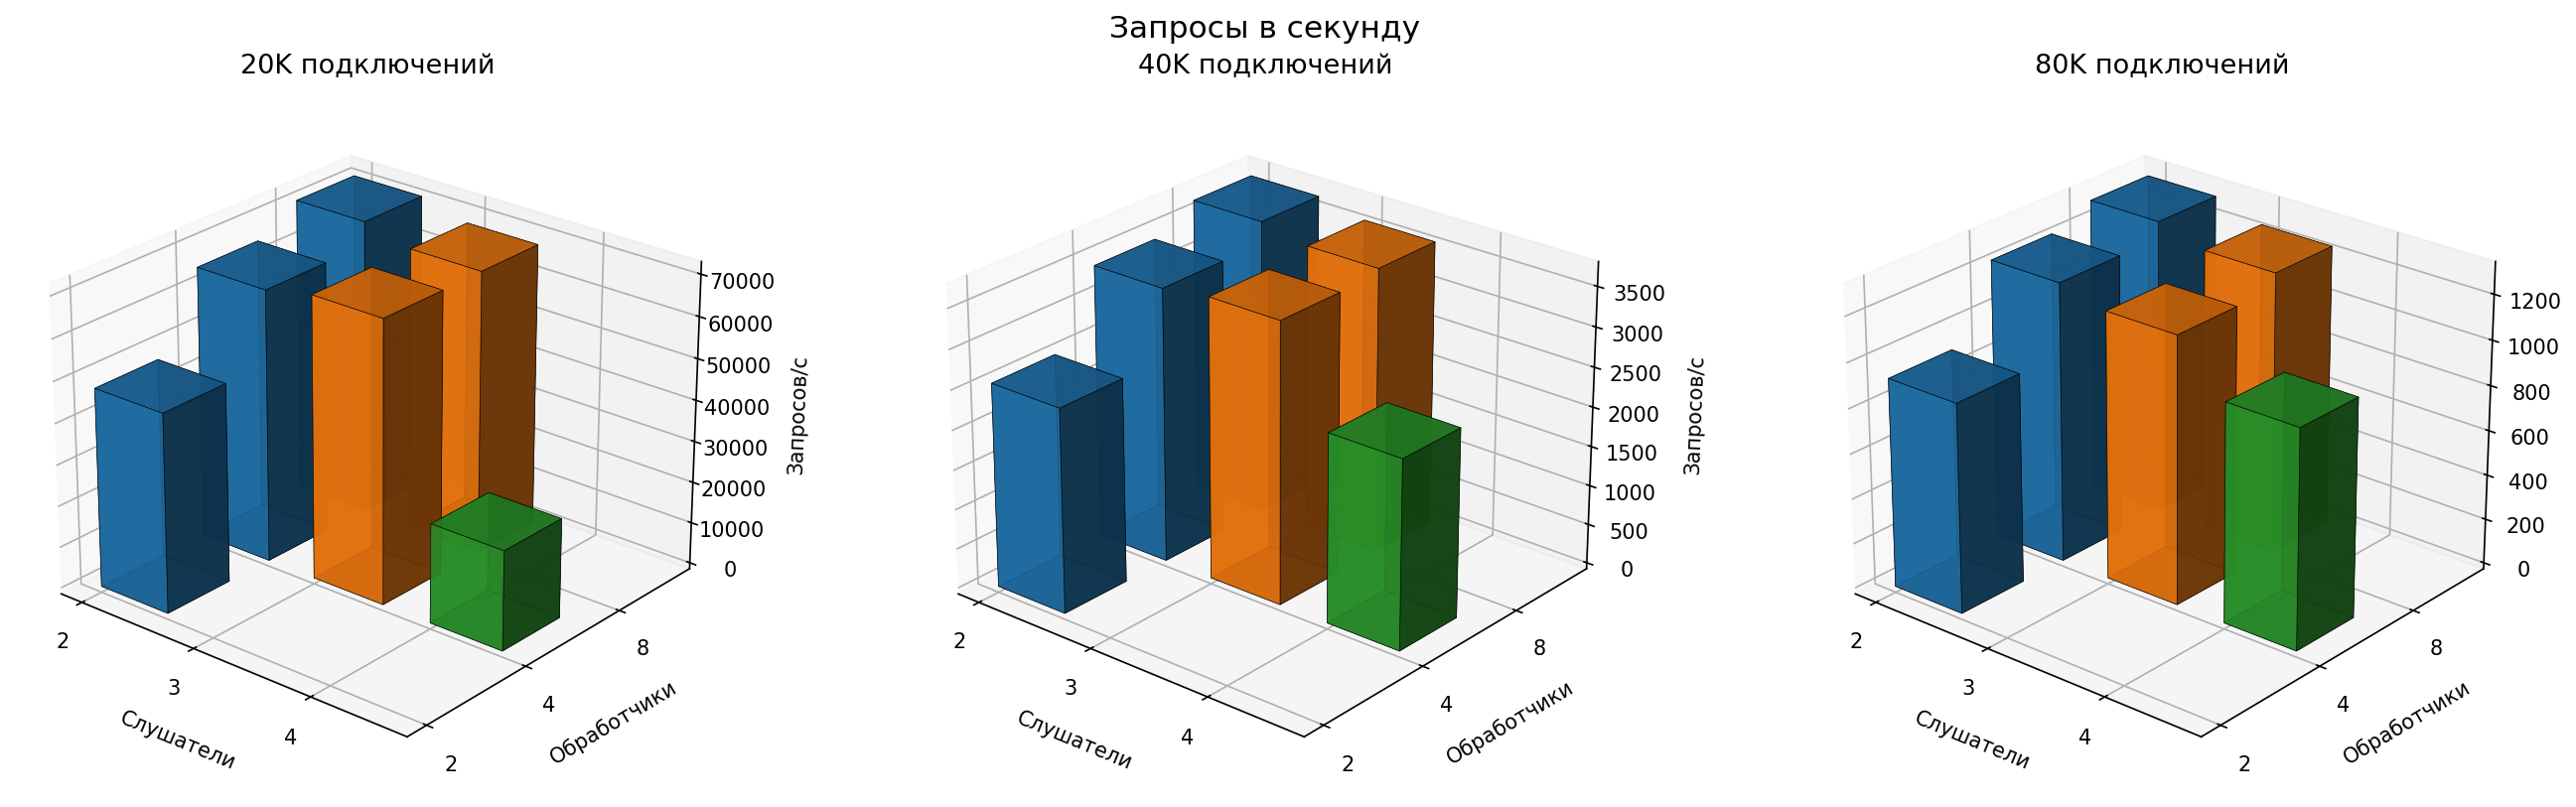
\includegraphics[width=\textwidth]{inc/img/3d_rps.png}}
	\caption{Зависимость пропускной способности от конфигурации потоков}
	\label{fig:3d_rps}
\end{figure}


\section{Исследование влияния количества потоков на задержку}
На рисунке~\ref{fig:3d_latency} представлена зависимость
средней задержки ответа от конфигурации потоков.

\begin{figure}[H]
	\center{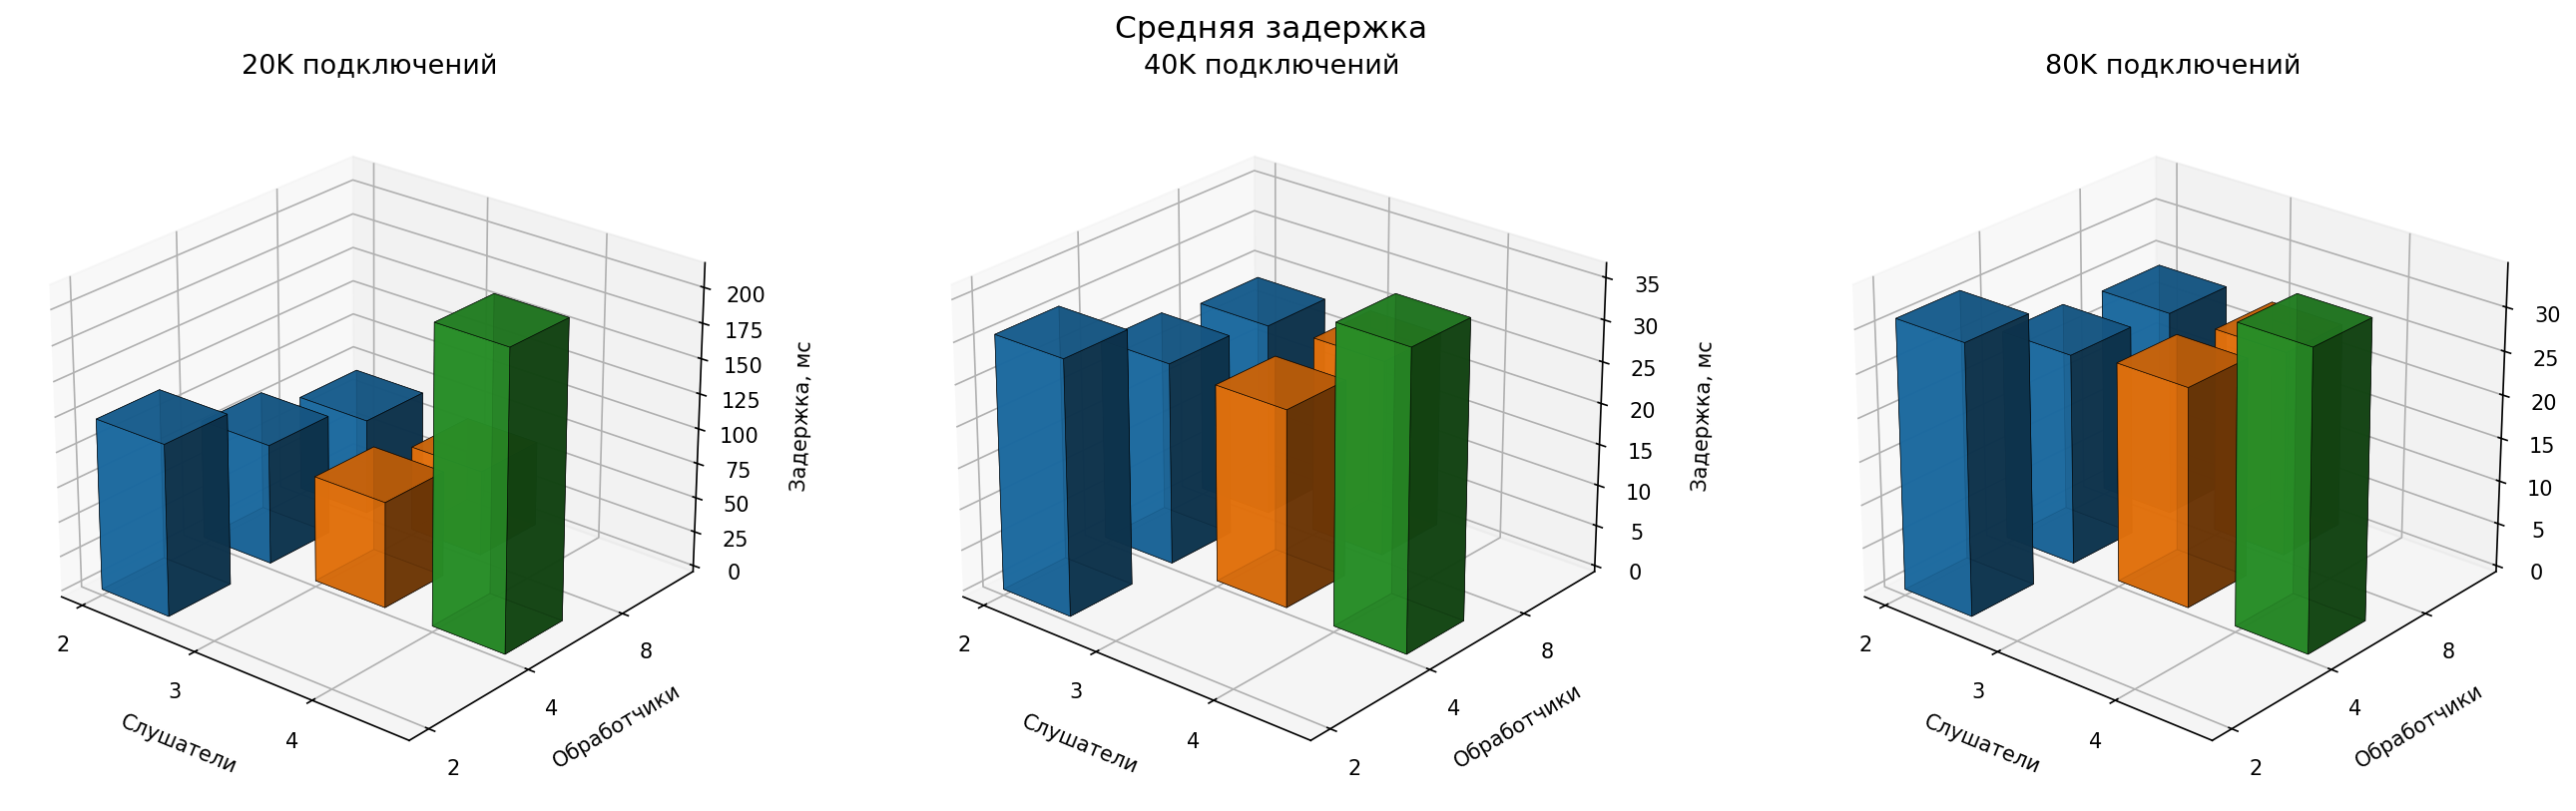
\includegraphics[width=\textwidth]{inc/img/3d_latency.png}}
	\caption{Зависимость средней задержки от конфигурации потоков}
	\label{fig:3d_latency}
\end{figure}


\section{Исследование влияния количества потоков на скорость передачи}
На рисунке~\ref{fig:3d_transfer} представлена зависимость
скорости передачи данных от конфигурации потоков.

\begin{figure}[H]
	\center{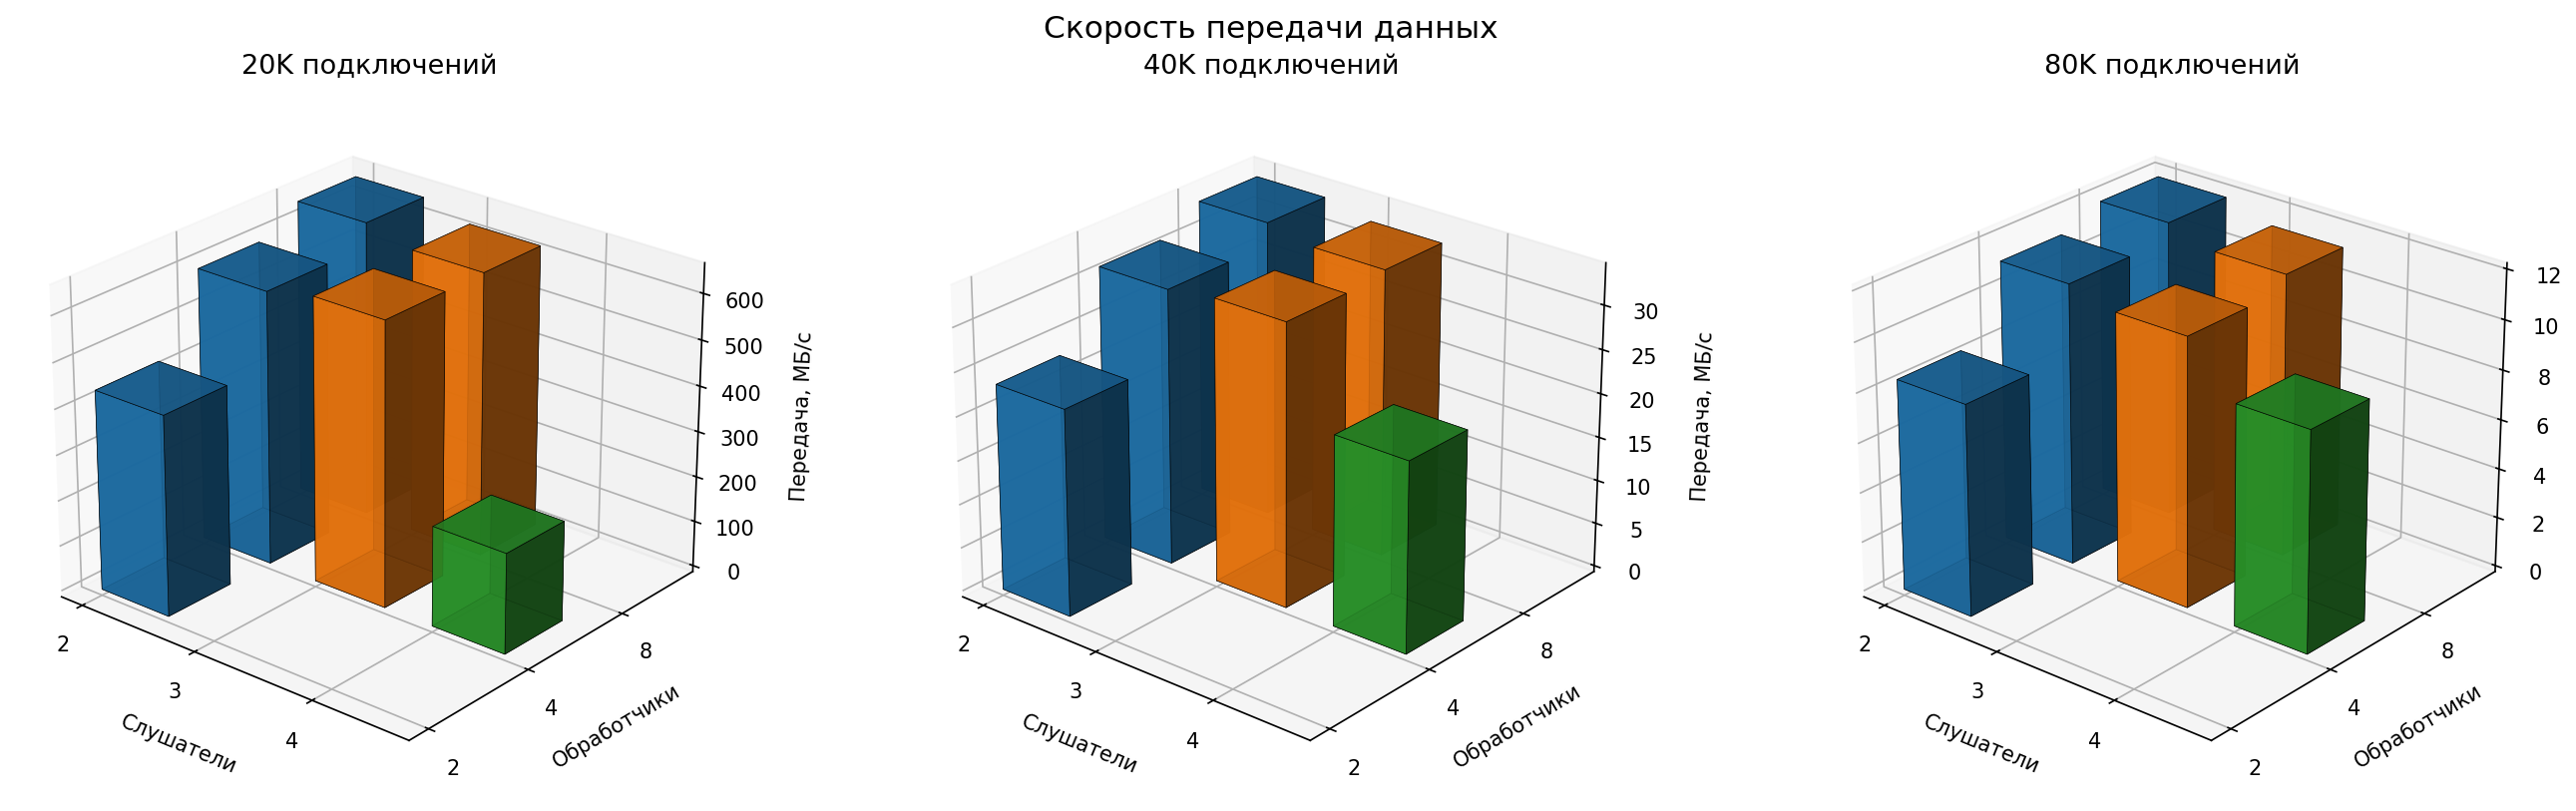
\includegraphics[width=\textwidth]{inc/img/3d_transfer.png}}
	\caption{Зависимость скорости передачи данных от конфигурации потоков}
	\label{fig:3d_transfer}
\end{figure}

\section{Исследование конфигурации $L{=}2$, $W{=}8$}
На рисунке~\ref{fig:cfg28_3d} представлена трёхмерная зависимость
задержки и скорости передачи от числа подключений
для конфигурации $(L{=}2,\,W{=}8)$,
аппроксимированная полиномом третьей степени.

\begin{figure}[H]
	\center{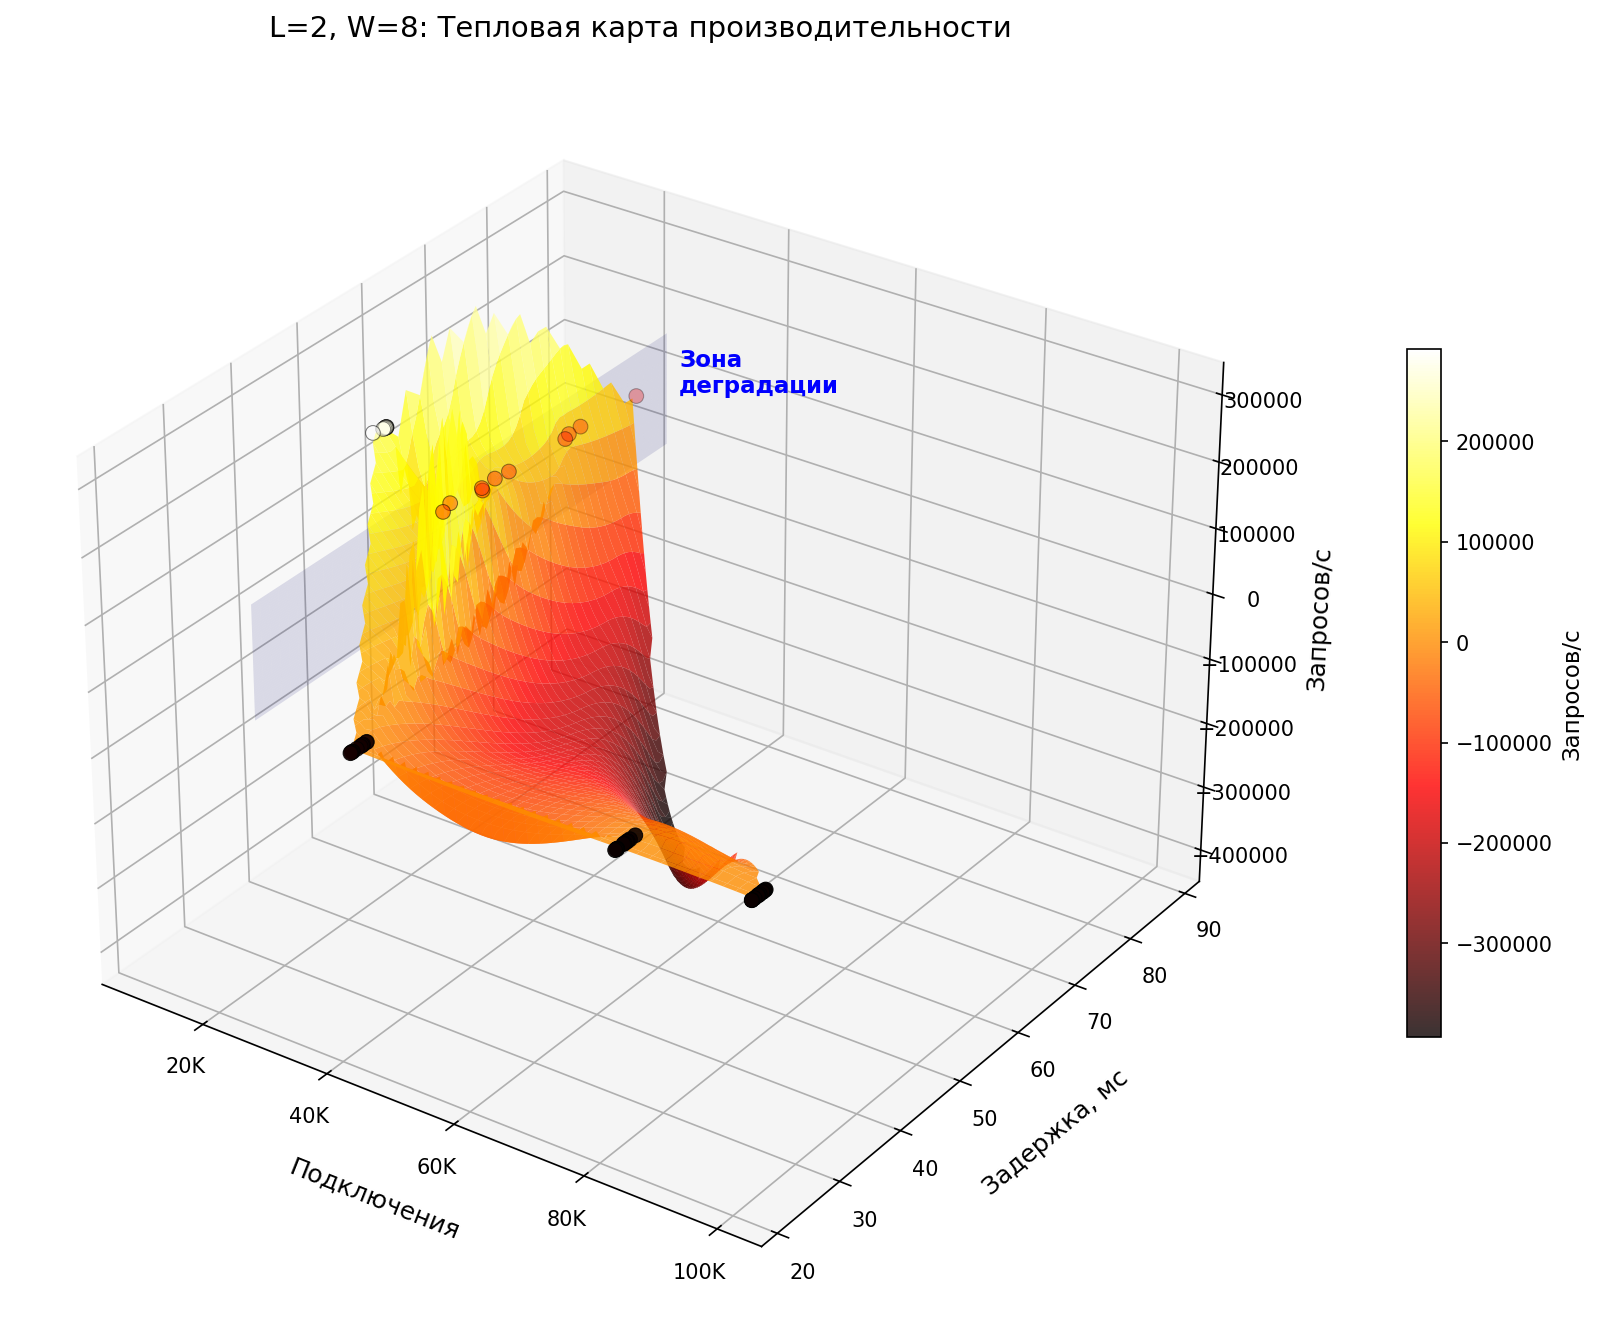
\includegraphics[width=0.85\textwidth]{inc/img/cfg_2_8_conn_lat_transfer_3d.png}}
	\caption{Конфигурация $L{=}2$, $W{=}8$: зависимость задержки и скорости передачи от числа подключений}
	\label{fig:cfg28_3d}
\end{figure}


\section{Выводы}
По результатам нагрузочного тестирования установлено следующее.

\begin{enumerate}
	\item Увеличение количества потоков-обработчиков оказывает
	наибольшее влияние на производительность сервера.
	При фиксированном числе слушателей $L{=}2$ увеличение
	числа обработчиков с 2 до 8 повышает пропускную способность
	на 77\% (с 95\,247 до 168\,414~req/s при 10\,000 подключений)
	и снижает задержку на 43\% (с 99,15 до 56,79~мс).

	\item Увеличение количества потоков-слушателей
	свыше двух не приводит к росту производительности.
	Конфигурация $(L{=}4,\,W{=}4)$ показала результаты
	в 2-3 раза хуже, чем $(L{=}2,\,W{=}4)$,
	что объясняется избыточной конкуренцией слушателей
	за входящие соединения при использовании \texttt{SO\_REUSEPORT}.

	\item При нагрузках свыше 40\,000+ подключений
	различия между конфигурациями нивелируются:
	узким местом становятся системные ограничения ОС,
	а не архитектура пула потоков.

	\item Оптимальной конфигурацией сервера
	является $(L{=}2,\,W{=}8)$.
	Данная конфигурация обеспечивает наибольшую пропускную
	способность и наименьшую задержку на всех
	уровнях нагрузки.
\end{enumerate}
